\documentclass[11pt,a4paper]{article}
\usepackage[margin=22mm]{geometry}
\usepackage{amsmath,amssymb}
\usepackage{booktabs,tabularx,array}
\usepackage{tikz}
\usetikzlibrary{arrows.meta,positioning,shapes.geometric}
\usepackage[hidelinks]{hyperref}
\usepackage{xcolor}
\setlength{\parskip}{4pt}
\newcommand{\st}[1]{\textsc{#1}}
\newcommand{\file}[1]{\texttt{#1}}
\title{Pathfinder as a state machine}
\author{Pathfinder, \file{github.com/vd1/pathfinder}}
\date{12 September 2026}
\begin{document}
\maketitle

\noindent One pair of papers is one machine. The campaign is a set of these machines plus a
scheduler with a purse. Everything below is what the code does; the builder prompt points here
for the shape to re-implement.

\section{Global state of a pair}

\paragraph{Position.} \file{stage}, where the machine is; \file{status}, one of \file{running},
\file{stopped}, \file{BLOCKED} or a terminal word; the counters \file{round} (research rounds
used), \file{repairs} (note repairs used), the paper's \file{round} and the editor's
\file{attempt}.

\paragraph{Memory,} all files under \file{threads/<pair>/}:
\begin{itemize}\setlength{\itemsep}{1pt}
  \item \file{inputs/}: the two papers, flattened \TeX{} or PDF text, and their metadata.
  \item \file{ledger.jsonl}: append-only attributed entries of kind idea, finding, objection,
    correction, intention, ready or review; the peers' shared memory and the verifier's evidence.
  \item \file{ada/}, \file{emmy/}, \ldots: each peer's derivations, scripts and checks.
  \item \file{<pair>.tex}: the consolidated note; \file{<pair>.verdict.json}: every verdict with
    the digest of the note it judged.
  \item \file{edited/}: the readable note (\file{note.tex}, \file{references.bib},
    \file{note.pdf}).
  \item \file{paper/}: the paper, its search record and every review with the digest of the paper
    it judged.
  \item \file{status.json}, \file{paper/paper.json}, \file{edited/edit.json}: the position.
\end{itemize}

\paragraph{Campaign level.} \file{scan.jsonl}, \file{shortlist.json}, \file{receipts.jsonl}
(the only spend figure), the markers \file{stop.json} and \file{health.json}, and one pid lock
per pair.

\section{States}

\begin{center}
\resizebox{\textwidth}{!}{%
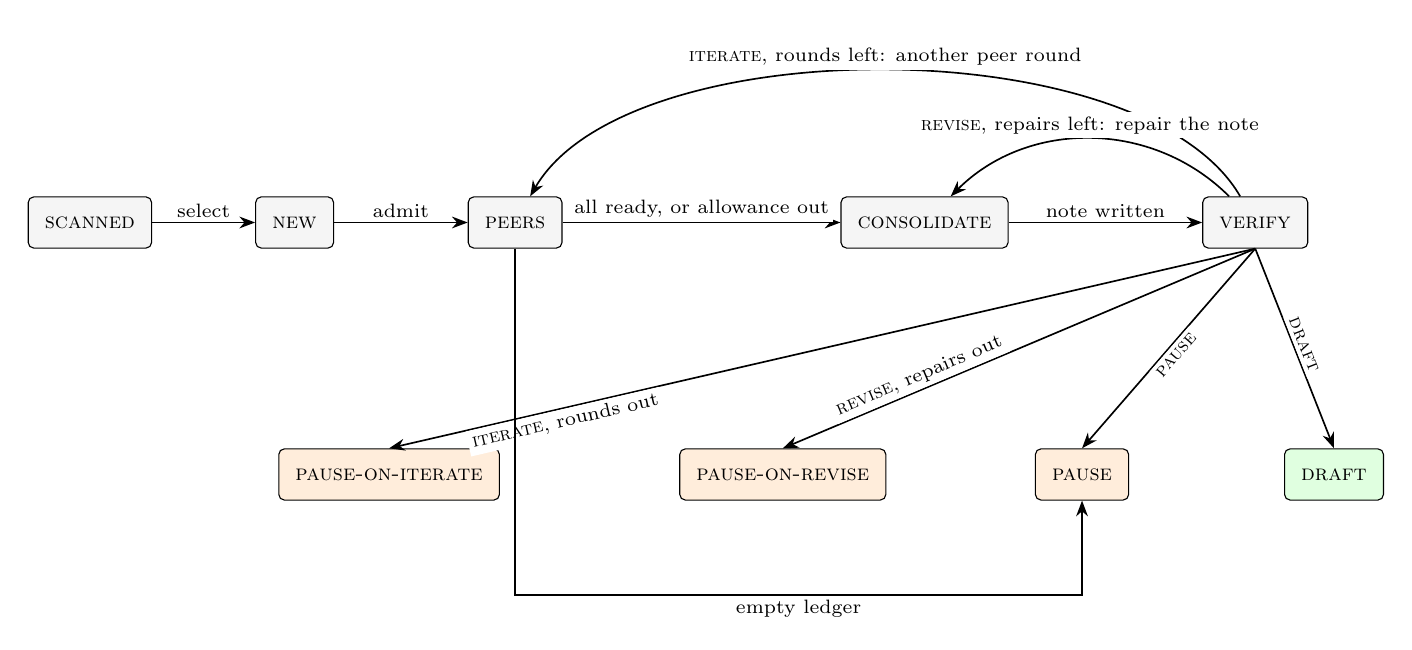
\begin{tikzpicture}[x=1cm, y=1cm,
  every node/.style={font=\footnotesize},
  state/.style={draw, rounded corners=2pt, minimum height=6.5mm, inner xsep=6pt, fill=gray!8},
  term/.style={state, fill=green!12},
  pause/.style={state, fill=orange!14},
  edge/.style={-{Stealth[length=2mm]}, semithick},
  lab/.style={font=\scriptsize, fill=white, inner sep=1.5pt}]
  \node[state] (scan) at (0.8,0) {\st{scanned}};
  \node[state] (new) at (3.4,0) {\st{new}};
  \node[state] (peers) at (6.2,0) {\st{peers}};
  \node[state] (cons) at (11.4,0) {\st{consolidate}};
  \node[state] (ver) at (15.6,0) {\st{verify}};
  \node[pause] (poi) at (4.6,-3.2) {\st{pause-on-iterate}};
  \node[pause] (por) at (9.6,-3.2) {\st{pause-on-revise}};
  \node[pause] (pause) at (13.4,-3.2) {\st{pause}};
  \node[term] (draft) at (16.6,-3.2) {\st{draft}};
  \draw[edge] (scan) -- node[lab, above] {select} (new);
  \draw[edge] (new) -- node[lab, above] {admit} (peers);
  \draw[edge] (peers) -- node[lab, above] {all ready, or allowance out} (cons);
  \draw[edge] (cons) -- node[lab, above] {note written} (ver);
  \draw[edge] (ver) to[out=120, in=60, looseness=0.7] node[lab, above] {\st{iterate}, rounds left: another peer round} (peers);
  \draw[edge] (ver) to[out=135, in=45, looseness=1.0] node[lab, above] {\st{revise}, repairs left: repair the note} (cons);
  \draw[edge] (ver.south) -- node[lab, sloped, above, pos=0.5] {\st{draft}} (draft.north);
  \draw[edge] (ver.south) -- node[lab, sloped, below, pos=0.5] {\st{pause}} (pause.north);
  \draw[edge] (ver.south) -- node[lab, sloped, above, pos=0.7] {\st{revise}, repairs out} (por.north);
  \draw[edge] (ver.south) -- node[lab, sloped, below, pos=0.8] {\st{iterate}, rounds out} (poi.north);
  \draw[edge] (peers.south) -- ++(0,-4.4) -| node[lab, pos=0.25, below] {empty ledger} (pause.south);
\end{tikzpicture}}

\medskip

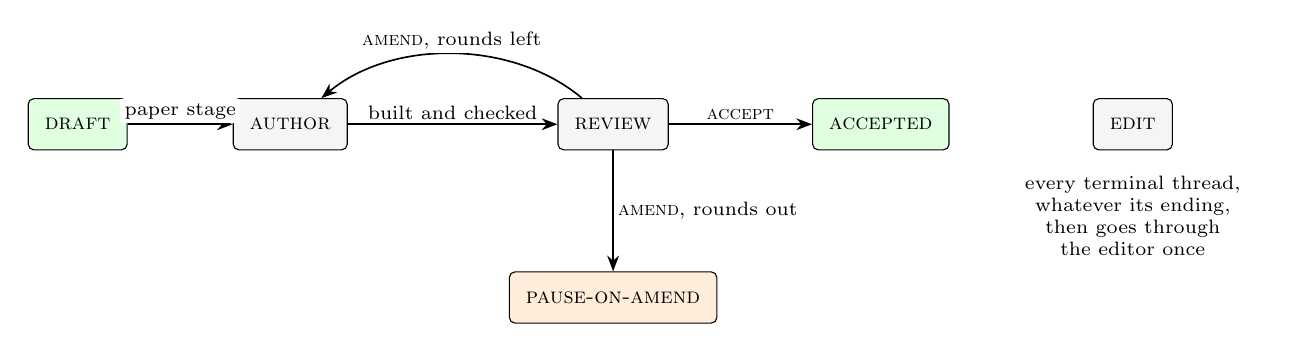
\begin{tikzpicture}[x=1cm, y=1cm,
  every node/.style={font=\footnotesize},
  state/.style={draw, rounded corners=2pt, minimum height=6.5mm, inner xsep=6pt, fill=gray!8},
  term/.style={state, fill=green!12},
  pause/.style={state, fill=orange!14},
  edge/.style={-{Stealth[length=2mm]}, semithick},
  lab/.style={font=\scriptsize, fill=white, inner sep=1.5pt}]
  \node[term] (draft) at (0.8,0) {\st{draft}};
  \node[state] (author) at (3.5,0) {\st{author}};
  \node[state] (review) at (7.6,0) {\st{review}};
  \node[term] (acc) at (11.0,0) {\st{accepted}};
  \node[pause] (poa) at (7.6,-2.2) {\st{pause-on-amend}};
  \node[state] (edit) at (14.2,0) {\st{edit}};
  \draw[edge] (draft) -- node[lab, above] {paper stage} (author);
  \draw[edge] (author) -- node[lab, above] {built and checked} (review);
  \draw[edge] (review) -- node[lab, above] {\st{accept}} (acc);
  \draw[edge] (review) to[out=140, in=40, looseness=0.9] node[lab, above] {\st{amend}, rounds left} (author);
  \draw[edge] (review) -- node[lab, right] {\st{amend}, rounds out} (poa);
  \node[font=\scriptsize, text width=34mm, align=center, below=2mm of edit] {every terminal thread, whatever its ending, then goes through the editor once};
\end{tikzpicture}
\end{center}

\noindent Terminal words of the research thread: \st{draft}, \st{pause}, \st{pause-on-iterate},
\st{pause-on-revise}. Terminal words of the paper: \st{accepted}, \st{pause-on-amend}. Every
\st{pause-on-x} means ``the loop named X ran out of its budget with the judge still asking''; a
human can raise the budget and resume from the recorded stage. The editor runs once for every terminal
thread, whatever its ending. \file{stopped} and \file{BLOCKED} are not endings:
\file{stopped} is a drain checkpoint (a stop marker, a transport failure, a kill) and resumes at
the recorded stage; \file{BLOCKED} is an unreadable decision or a missing output and waits for
\file{reconcile}.

\section{Transitions}

Each transition is one or more model calls. ``Sees'' is the part of the global state the agent
can read; ``writes'' is what it may change. Nothing else is visible or writable, which is what
makes the record auditable.

\begin{small}
\begin{tabularx}{\textwidth}{@{}>{\raggedright\arraybackslash}p{19mm} >{\raggedright\arraybackslash}p{27mm} X X >{\raggedright\arraybackslash}p{34mm}@{}}
\toprule
from $\to$ to & agent, prompt, tools & sees & writes & budget \\
\midrule
corpus $\to$ \st{scanned} & judge, \file{scan.md}, no tools & Q and P titles and abstracts, or full text & one row of \file{scan.jsonl} & one call, retried once if unparseable \\
\st{scanned} $\to$ \st{new} & none (\file{select}) & all scan rows & \file{shortlist.json} & none \\
\st{new} $\to$ \st{peers} & none (runner) & shortlist, statuses, locks, receipts, markers & lock, \file{status.json} & seats; guard: spend plus in-flight estimate under \file{budget\_usd}, else the stop marker \\
\st{peers} $\to$ \st{peers} & every peer concurrently, \file{peer.md}, tools and web search & inputs, ledger, own and partners' directories, the scan's connexion and scores, this call's allowance & ledger entries through the helper, own directory & \file{peer\_calls} per peer and \file{peer\_seconds} shared, per round; a peer whose ready stands waits instead of calling \\
\st{peers} $\to$ \st{consolidate} & none & ledger readiness & \file{status.json} & when every peer is ready or the allowance is out; an empty ledger goes to \st{pause} \\
\st{consolidate} $\to$ \st{verify} & first peer, \file{consolidate.md}, tools & ledger, all directories, the prior note and the verifier's review if any & \file{<pair>.tex} & \file{consolidate\_seconds}; rerun once unless the note exists \\
\st{verify} $\to$ next & verifier, \file{verify.md}, no tools & inputs, ledger, note, all inline & verdict file, a review entry in the ledger, \file{status.json} & \file{verify\_seconds}; rerun once on an empty reply \\
\st{verify} $\to$ \st{peers} & verdict \st{iterate} & & \file{round} $+1$ & \file{rounds} (4); at the cap \st{pause-on-iterate} \\
\st{verify} $\to$ \st{consolidate} & verdict \st{revise} & the consolidator also sees the corrections & \file{repairs} $+1$ & \file{repairs} (1); at the cap \st{pause-on-revise} \\
\st{draft} $\to$ \st{review} & author, \file{author.md}, tools and web search & everything in the thread, the web, the previous review's findings if any & \file{paper/} & \file{paper\_seconds} per call \\
\st{review} $\to$ next & reviewer, \file{review.md}, no tools & paper, bib, the pipeline's reference checks, the search record, note, ledger, inputs, all inline & \file{paper/review.json}, \file{paper.json} & \file{review\_seconds}; \file{paper\_rounds} (3); at the cap \st{pause-on-amend} \\
terminal $\to$ \st{edit} & editor, \file{editor.md}, tools, no search & inputs and metadata, note, verdicts, ledger, all directories, the build and reference checks on retry & \file{edited/} & \file{edit\_seconds}; two attempts, then \file{blocked} \\
\bottomrule
\end{tabularx}
\end{small}

\medskip\noindent Between transitions the pipeline itself, with no model, does the checks that
gate the next state: it builds the \LaTeX, verifies citations against the bibliography and
arXiv, records digests, and writes the position. The verifier's and reviewer's judgements are
the only decisions; every other arrow is mechanical.

\section{Budgets, and what exhausting them means}

\begin{center}
\begin{tabular}{@{}lll@{}}
\toprule
budget & scope & when exhausted \\
\midrule
\file{peer\_calls}, \file{peer\_seconds} & one peer round & consolidate on the ledger as it stands \\
\file{rounds} & the \st{iterate} loop & \st{pause-on-iterate} \\
\file{repairs} & the \st{revise} loop & \st{pause-on-revise} \\
\file{paper\_rounds} & the \st{amend} loop & \st{pause-on-amend} \\
editor attempts & the build and reference checks & \file{blocked} \\
\file{budget\_usd} & the campaign, at admission & stop marker; threads in flight finish; \st{new} pairs wait \\
\bottomrule
\end{tabular}
\end{center}

\noindent Every model call appends a receipt, so the campaign budget is checked against the sum
of receipts, never against an estimate alone.

\section{Interrupts}

\begin{itemize}\setlength{\itemsep}{1pt}
  \item A stop marker (operator, guard, or first Ctrl-C) stops admission; calls in flight land
    and write their checkpoints; the runner exits; the next start resumes each pair at its
    recorded stage.
  \item No session within the grace time is a transport failure: no receipt, the pair is
    \file{stopped}, two in a row set the health marker and pause admission until a probe
    succeeds.
  \item \file{reconcile} reads the position of one pair and names the one safe action: start,
    resume peers, run consolidate, run verify, or nothing; \file{--apply} performs it.
\end{itemize}
\end{document}
